\chapter{Incentives and Truthfulness}
\label{cha:incentives_and_truthfulness}

\begin{figure}
    \centering
    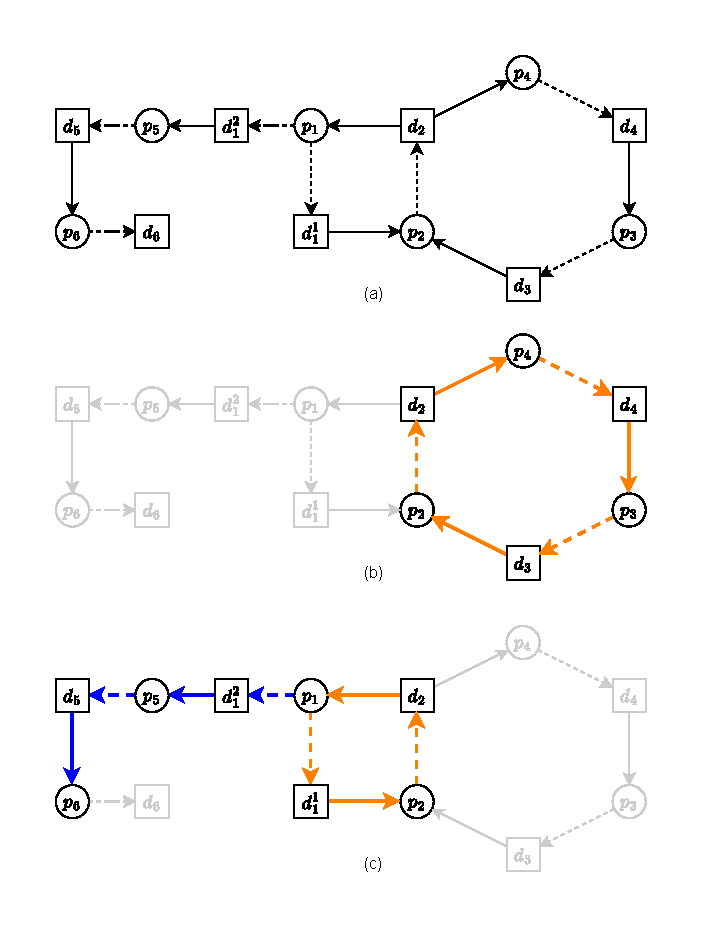
\includegraphics{data/incentive_motivation_example.pdf}
    \caption[An example showing the difference between alternative-donors model and multiple-donors model]{\textbf{(a)} shows an example of a graph containing two overlapping cycles, where the left cycle contains patient $p_1$ which has two proxy donors: $d_1^1$ and $d_1^2$. \textbf{(b)} shows the output of the alternative-donors model. \textbf{(c)} shows the output of the multiple-donors model.}
    \label{fig:incentive_motivation_example}
\end{figure}


\begin{figure}
    \centering
    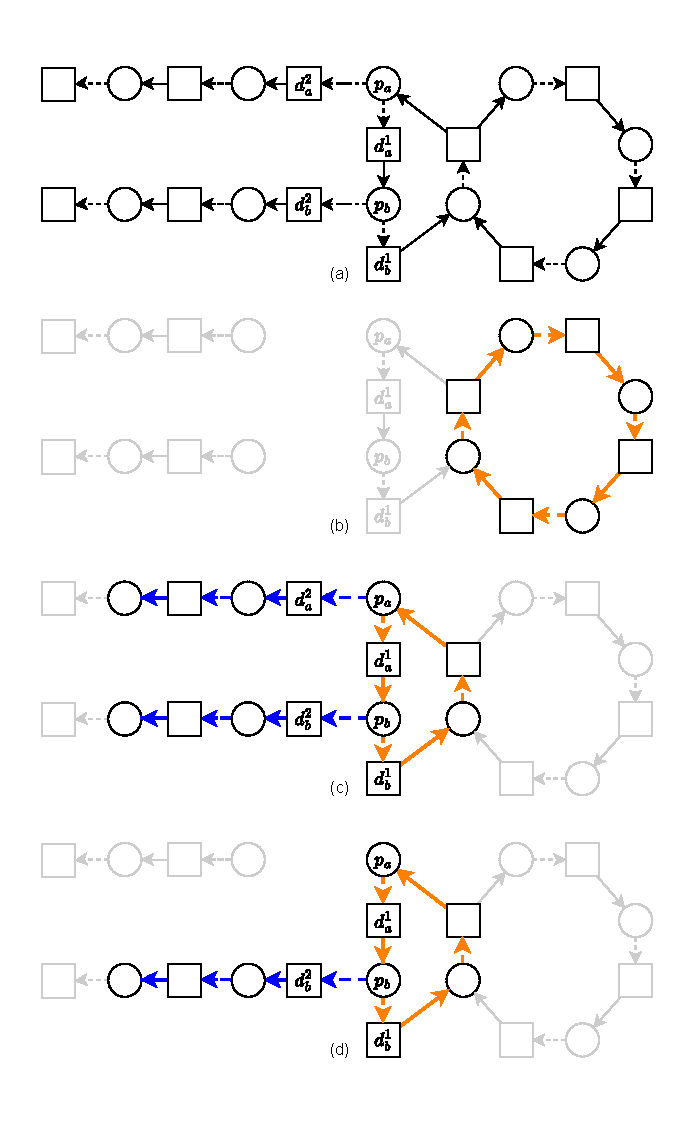
\includegraphics{data/prisoners_dilemma.pdf}
    \caption[Prisoner's dilemma in multiple-donors model]{\textbf{(a)} illustrates a graph where patients $p_a$ and $p_b$ are in \textit{Prisoner's Dilemma} situation. \textbf{(b)} shows that if both $p_a$ and $p_b$ decide not to report $d_a^2$ and $d_b^2$ respectively, they both don't receive compatible kidney in the final solution. In \textbf{(c)}, both patients reported both of theirs donors, they both receive compatible kidney but also they both spent two kidneys of their proxy donors. In \textbf{(d)}, patient $p_b$ reported both of his proxy donors, patient $p_a$ reported only $d_a^1$. In this case, $p_a$ gets a compatible kidney and spends only one proxy kidney. Patient $p_b$ gets a compatible kidney as well but spends two proxy kidneys. The symmetric occurs when $p_a$ reports two proxy donors and $p_b$ reports only one of his proxies.}
    \label{fig:prisoners_dilemma}
\end{figure}


%%% Local Variables:
%%% mode: latex
%%% TeX-master: "../ClassicThesis"
%%% ispell-dictionary: "british" ***
%%% fill-column: 76 ***
%%% End:
